\documentclass{pset}

\renewcommand{\hmwkTitle}{5th\ week\ hw}
\renewcommand{\hmwkDueDate}{February 12, 2014}
\renewcommand{\hmwkClass}{Measure Theory}
\renewcommand{\hmwkClassTime}{Chapter 2}
\renewcommand{\hmwkAuthorName}{}

%
% Title Page
%

\title{
    \vspace{2in}
    \textmd{\textbf{\hmwkClass:\ \hmwkTitle}}\\
    \normalsize\vspace{0.1in}\small{Due\ on\ \hmwkDueDate\ at 3:10pm}\\
    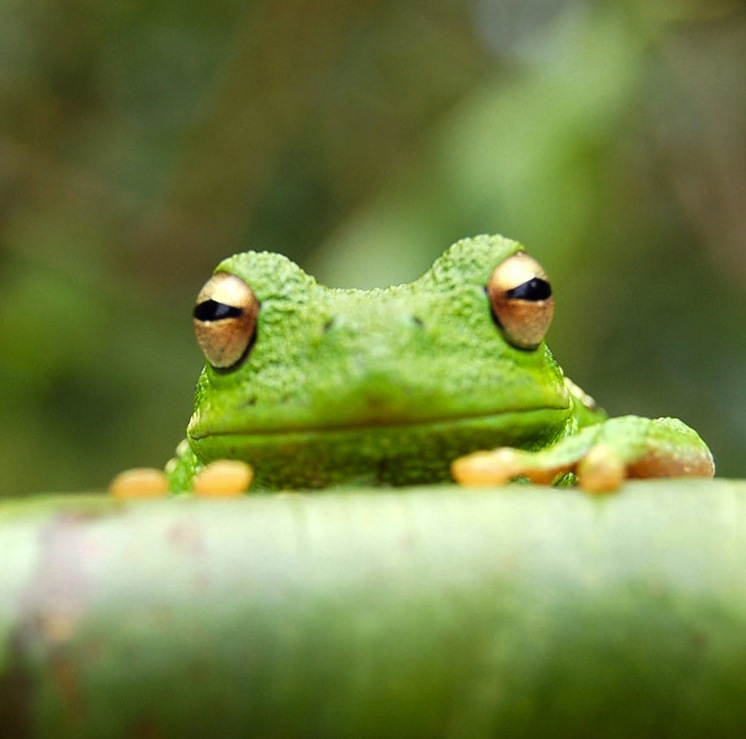
\includegraphics[scale=0.2]{frog} \\
    \vspace{0.1in}\large{\textit{\hmwkClassTime}}
    \vspace{3in}
}

\author{\hmwkAuthorName}
\date{}

\renewcommand{\part}[1]{\textbf{\large Part \Alph{partCounter}}\stepcounter{partCounter}\\}

% Integral dx  
\newcommand{\dx}{\mathrm{d}x}

\begin{document}

\maketitle

\pagebreak 
\begin{problem}
    \begin{enumerate}[label=\alph*.]
        \item 
        \begin{enumerate}
            \item $\nu(\varnothing)=\mu(T^{-1}(\varnothing))=\mu(\varnothing)=0$
            \item let $\{E_i\}_{i=0}^\i$ be a sequence of disjoint sets in $\mcl{M}_Y$
            \begin{align}
                \nu\biggl(\bigcup_{i=0}^\i E_i\biggr) &= \mu\biggl(T^{-1}\biggl(\bigcup_{i=0}^\i E_i\biggr)\biggr) \\
                &= \mu\biggl(\bigcup_{i=0}^\i T^{-1}(E_i)\biggr) \\
                &= \sum_{i=0}^\i\mu\big(T^{-1}(E_i)\big) \\
                &= \sum_{i=0}^\i \nu(E_i)
            \end{align}
            (1) and (4) follow from definition of $\nu$, (2) follows from properties of preimages and (3) is justified coz the preimage of disjoint sets is disjoint.
        \end{enumerate}
        \item First note that $f$ is measurable iff $f\circ T$ is measurable. We then prove the statement for characteristic functions first: suppose $f=\Chi_E$ where $E\in \mcl{M}_Y$ but note that $f\circ T$ is also a characteristic function and
        \[(f\circ T)^{-1}(1)=T^{-1}\bigl(f^{-1}(1)\bigr)=T^{-1}(E)\]
        which means $f\circ T = \Chi_{T^{-1}(E)}$ and hence
        \[\int f\circ T\dd\mu = \int \Chi_{T^{-1}(E)}\dd\mu = \mu(T^{-1}(E)) = \nu(E) = \int f\dd\nu\]
        and hence the statement is true for characteristic functions and also simple functions by linearity. Now for the general case let $\{\phi_i\}$ be an increasing sequence of simple functions that converge to $f$ a.e. so by applying the MCT we get
        \[\int f\dd\nu = \lim_{i\to\i}\int \phi_i\dd\nu = \lim_{i\to\i}\int \phi_i\circ T\dd\mu = \int f\circ T\dd\mu\]
    \end{enumerate}
\end{problem}
\begin{problem}[33]
    suppose $\int f\geq \liminf\int f_n$, that means there exists a subsequence $\{f_{n_k}\}_{k=0}^\i$ such that $\liminf\int f_n=\lim \int f_{n_k}$ but the subsequence obviously still converges to $f$ in measure so it must contain a subsubsequence $\{f_{n_{k_j}}\}_{j=0}^\i$ that converges to $f$ pointwise a.e. but using Fatou's lemma we see that
    \[
        \int f\leq \liminf_{j\to\i} \int f_{n_{k_j}} = \lim_{k\to\i} \int f_{n_k} = \liminf_{n\to\i} \int f_n
    \]
    which would mean
    \[
        \int f = \liminf_{n\to\i}\int f_n
    \]
\end{problem}
\begin{problem}
    \begin{enumerate}[label=\alph*.]
        \item $f$ is measurable since it's the limit of some subsequence of $\{f_n\}$ which are all measurable functions and it's integrable since $f=\lim f_n\leq g$. Now we note that $f_n+g\geq 0$ and $g-f_n\geq 0$ and both sequences converge in measure to $f+g$ and $g-f$ respectively so we can use the previous problem to conclude that
        \begin{align*}
            \int g + \int f &\leq \liminf \int (g+f_n) = \int g + \liminf \int f_n \\
            \int g - \int f &\leq \liminf \int (g-f_n) = \int g - \limsup \int f_n
        \end{align*}
        from which $\limsup \int f_n\leq \int f\leq \liminf \int f_n$ and hence we're done
        \item we have $\abs{f-f_n}\leq 2g$ and it's fairly evident that $\abs{f-f_n}\to 0$ in measure and hence, by using (a), we see that
        \[
            \lim_{n\to\i}\int\abs{f-f_n}=0
        \]
    \end{enumerate}
\end{problem}
\begin{problem}[40]
    It suffices to prove that $E_n(k)$, as defined in the orginal proof, are eventually finite. Indeed, according to the DCT, $f_n\to f$ in $L^1$ but if $E_n(k)$ \emph{aren't} eventually finite then 
    \[\int \abs{f_n-f}\geq \int_{E_n(k)}\abs{f_n-f}\geq \int_{E_n(k)}\frac{1}{k} = \i\]
    which is a contradiction. 
\end{problem}
\begin{problem}[44]
    Let $\eps>0$. We're going to prove the result for postive real functions first. Notice that
    \[\sum_{i=0}^\i\mu\big(f^{-1}\big([i, i+1)\big)\big)=\mu([a, b])\]
    is a convergent sequence which means there exists an $N\in\bN$ such that
    \[\sum_{i=N}^\i\mu\big(f^{-1}\big([i, i+1)\big)\big)=\mu\big(f^{-1}([N, +\i))\big)<\eps\]
    that means that, if $E_1=f^{-1}([0, N))$, then $f_{E_1}\in L^1$ and $\mu(E_1^c)<\eps$.

    Now using problem 3 from the last hw, we know that there must exist a sequence of continuous functions $\{f_n\}$ that converges a.e. to $f$ in $E_1$ and using egoroff's there must exist a set $E_2$ such that $\mu(E_2^c)<\eps$ and $\{f_n\}$ converges uniformly on $E_2$. And using inner regularity we can find a compact set $E_2'$ such that $\mu(E_2\setminus E_2')<\eps$ which means $\mu(E_2'^c)<2\eps$ and $\{f_n\}$ is still converges uniformly on $E_2'$ which means the restriciton of its limit to $E_2'$ is continuous. Now just put $E=E_1\cap E_2'$ and we can see that $f_|E$ is continuous and it's easy to check that $\mu(E)<3\eps$.

    Now for the general case, we can decompose $f$ as $f=(g^+-g^-)+i(h^+-h^-)$ where $g^+,g^-,h^+,h^-$ are all positive functions from which we can extract sets $E_1, E_2, E_3, E_4$ on the intersection of which all our functions (hence $f$ as well) are continuous and
    \[\mu\biggl(\bigcup_1^4 E_i\biggr)<4\cdot \frac{\eps}{4}=\eps\]
\end{problem}
\begin{problem}[52]
    (for convennience, let's order the elements in $Y=\{y_i\}_{i=0}^\i$)
    
    First we note that it is evident that if $g\in L^+(\nu)$ then
    \[\int g\dd\nu = \sum_{i=0}^\i g(y_i)\]
    and if $f\in L^+(\mu\times\nu)$ then for any $y\in Y$
    \[\int \Chi_{X\times \{y\}} \cdot f\dd\mu\times\nu = \int f^y\dd\mu\]
    (it's easy to see that this holds for characteristic funcitons and from that, by applying the MCT, you get the general case) now suppose $f\in L^1(\mu\times\nu)$, not that $f=\lim_{n\to\i}\sum_{i=0}^n \Chi_{X\times \{y_i\}}f$ and by using the MCT we see that
    \begin{align*}
        \int f \dd\mu\times\nu &= \sum_{i=0}^\i\int \Chi_{X\times \{y_i\}} f\dd\mu\times\nu \\
        &= \sum_{i=0}^\i\int f^{y_i}\dd\mu \\
        &= \iint f^y\dd\mu\dd\nu
    \end{align*}
    and
    \begin{align*}
        \int f \dd\mu\times\nu &= \sum_{i=0}^\i\int \Chi_{X\times \{y_i\}} f\dd\mu\times\nu \\
        &= \sum_{i=0}^\i\int f^{y_i}(x)\dd\mu(x) \\
        &= \int \sum_{i=0}^\i f^{y_i}(x)\dd\mu(x) \\
        &= \iint f_x\dd\nu\dd\mu
    \end{align*}
    This establishes Tonelli 's theorem and also shows that if $f\in L^+(\mu\times\nu)$ and $\int f<\i$, then $\int f_x\dd\nu<\i$ a.e. and $\int f^y\dd\mu<\i$ a.e., that is, $f_x\in L^1(\nu)$ for a.e. $x$ and $f^y \in L^1(\mu)$ for a.e. $y$. If $f\in L^1(\mu\times\nu)$, then, the conclusion of Fubini's theorem follows by applying these results to the positive and
negative parts of the real and imaginary parts of f. 
\end{problem}

\end{document}
